\section{Theorie}
\label{sec:Theorie}

In diesem Versuch wird das Relaxationsverhalten eines RC-Kreises untersucht.
Relaxation beschreibt allgemein die nicht-oszillatorische Rückkehr eines Systems in seinen Ausgangszustand.
Die Änderung der betrachteten Größe ist meistens proportional zur Zeit $t$, somit ergibt sich eine asymptotische
Annährung an den Ausgangszustand.

\subsection{Auf- und Entladen eines Kondensators}
Ein wichtiges Beispiel für Relaxationsvorgänge ist das Entladen eines zuvor aufgeladenen Kondensators im RC- Kreis.
Ein RC Kreis besteht aus einem Widerstand $R$ und einem Kondensator mit der Kapazität $C$ sowie einem Schalter, um zwischen 
Auf- und Entladen zu wechseln:

\begin{figure}
    \centering
    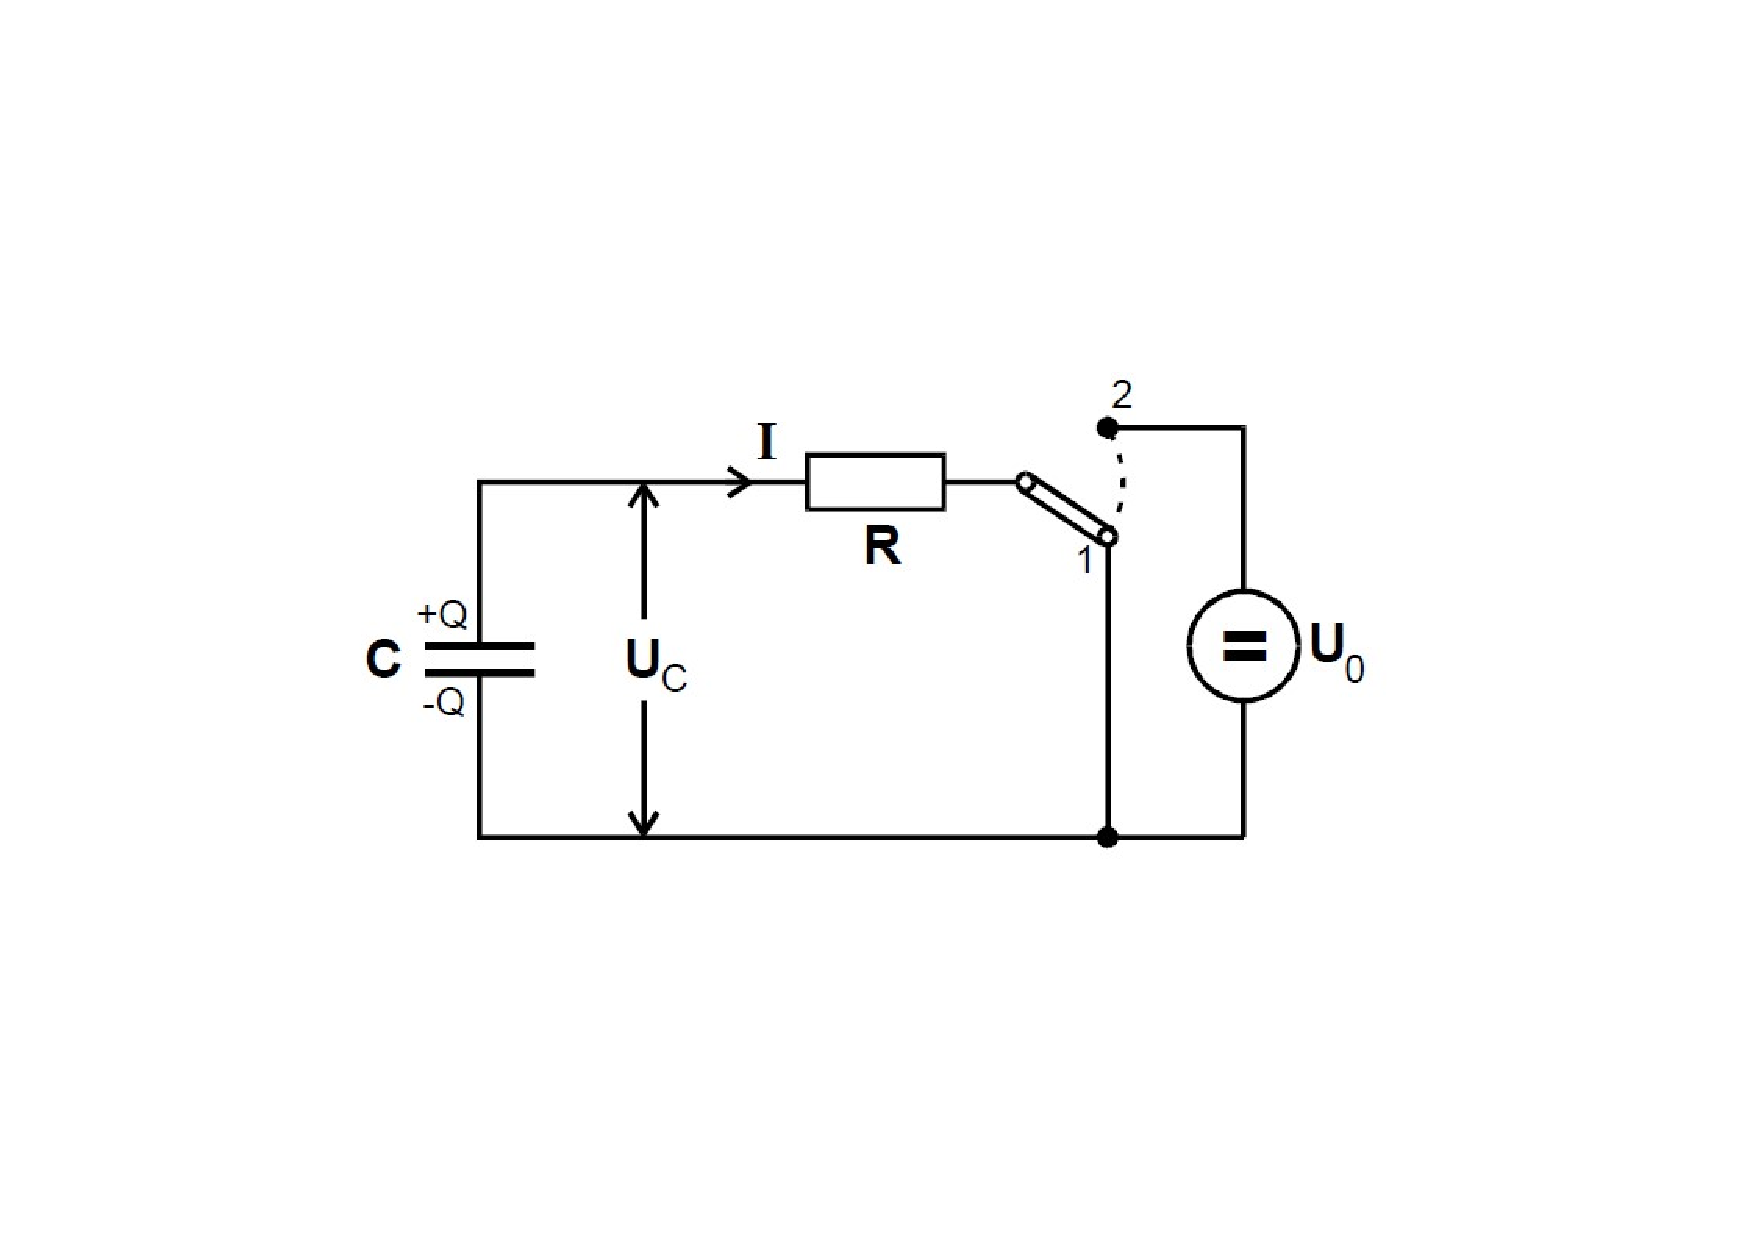
\includegraphics[height=10cm]{content/Theorie - RC-Kreis.pdf}
    \caption{RC Kreis mit Schalter}
    \label{fig:THeorie - RC_Kreis}
\end{figure}

Der Spannungsverlauf beim Entladen ist gegeben durch:

\begin{equation}
    U(t)= CU_{0}e^{-\frac{1}{RC}t} . \label{eqn:Entladen}
\end{equation}

Beim Aufladen lautet die Formel:

\begin{equation}
    U(t)= CU_{0}(1-e^{-\frac{1}{RC}t}) . \label{eqn:Aufladen}
\end{equation}

Dabei beschreibt $-\frac{1}{RC}$ die Zeitkonstante $c$, diese ist das Maß für die Geschwindigkeit mit der das System seinem
Ausgangszustand zustrebt und soll in diesem Versuch experimentell ermittelt werden.
Außerdem wird das öffnen7schließen des Schalters durch das anlegen einer Rechtecksspannung ersetzt.

\subsection{Relaxationsvorgänge bei periodischer Auslenkung, hier Tiefpass}



\cite{sample}

